\documentclass{article} % For LaTeX2e
\usepackage{iclr2024_conference,times}

% Stolen style files from ICLR 2024
% Optional math commands from https://github.com/goodfeli/dlbook_notation.
%%%%% NEW MATH DEFINITIONS %%%%%

\newcommand{\points}[1]{\texttt{\textbf{\textcolor{blue}{[#1 points]}}}}


\usepackage{amsmath,amsfonts,bm}

% Mark sections of captions for referring to divisions of figures
\newcommand{\figleft}{{\em (Left)}}
\newcommand{\figcenter}{{\em (Center)}}
\newcommand{\figright}{{\em (Right)}}
\newcommand{\figtop}{{\em (Top)}}
\newcommand{\figbottom}{{\em (Bottom)}}
\newcommand{\captiona}{{\em (a)}}
\newcommand{\captionb}{{\em (b)}}
\newcommand{\captionc}{{\em (c)}}
\newcommand{\captiond}{{\em (d)}}

% Highlight a newly defined term
\newcommand{\newterm}[1]{{\bf #1}}


% Figure reference, lower-case.
\def\figref#1{figure~\ref{#1}}
% Figure reference, capital. For start of sentence
\def\Figref#1{Figure~\ref{#1}}
\def\twofigref#1#2{figures \ref{#1} and \ref{#2}}
\def\quadfigref#1#2#3#4{figures \ref{#1}, \ref{#2}, \ref{#3} and \ref{#4}}
% Section reference, lower-case.
\def\secref#1{section~\ref{#1}}
% Section reference, capital.
\def\Secref#1{Section~\ref{#1}}
% Reference to two sections.
\def\twosecrefs#1#2{sections \ref{#1} and \ref{#2}}
% Reference to three sections.
\def\secrefs#1#2#3{sections \ref{#1}, \ref{#2} and \ref{#3}}
% Reference to an equation, lower-case.
\def\eqref#1{equation~\ref{#1}}
% Reference to an equation, upper case
\def\Eqref#1{Equation~\ref{#1}}
% A raw reference to an equation---avoid using if possible
\def\plaineqref#1{\ref{#1}}
% Reference to a chapter, lower-case.
\def\chapref#1{chapter~\ref{#1}}
% Reference to an equation, upper case.
\def\Chapref#1{Chapter~\ref{#1}}
% Reference to a range of chapters
\def\rangechapref#1#2{chapters\ref{#1}--\ref{#2}}
% Reference to an algorithm, lower-case.
\def\algref#1{algorithm~\ref{#1}}
% Reference to an algorithm, upper case.
\def\Algref#1{Algorithm~\ref{#1}}
\def\twoalgref#1#2{algorithms \ref{#1} and \ref{#2}}
\def\Twoalgref#1#2{Algorithms \ref{#1} and \ref{#2}}
% Reference to a part, lower case
\def\partref#1{part~\ref{#1}}
% Reference to a part, upper case
\def\Partref#1{Part~\ref{#1}}
\def\twopartref#1#2{parts \ref{#1} and \ref{#2}}

\def\ceil#1{\lceil #1 \rceil}
\def\floor#1{\lfloor #1 \rfloor}
\def\1{\bm{1}}
\newcommand{\train}{\mathcal{D}}
\newcommand{\valid}{\mathcal{D_{\mathrm{valid}}}}
\newcommand{\test}{\mathcal{D_{\mathrm{test}}}}

\def\eps{{\epsilon}}


% Random variables
\def\reta{{\textnormal{$\eta$}}}
\def\ra{{\textnormal{a}}}
\def\rb{{\textnormal{b}}}
\def\rc{{\textnormal{c}}}
\def\rd{{\textnormal{d}}}
\def\re{{\textnormal{e}}}
\def\rf{{\textnormal{f}}}
\def\rg{{\textnormal{g}}}
\def\rh{{\textnormal{h}}}
\def\ri{{\textnormal{i}}}
\def\rj{{\textnormal{j}}}
\def\rk{{\textnormal{k}}}
\def\rl{{\textnormal{l}}}
% rm is already a command, just don't name any random variables m
\def\rn{{\textnormal{n}}}
\def\ro{{\textnormal{o}}}
\def\rp{{\textnormal{p}}}
\def\rq{{\textnormal{q}}}
\def\rr{{\textnormal{r}}}
\def\rs{{\textnormal{s}}}
\def\rt{{\textnormal{t}}}
\def\ru{{\textnormal{u}}}
\def\rv{{\textnormal{v}}}
\def\rw{{\textnormal{w}}}
\def\rx{{\textnormal{x}}}
\def\ry{{\textnormal{y}}}
\def\rz{{\textnormal{z}}}

% Random vectors
\def\rvepsilon{{\mathbf{\epsilon}}}
\def\rvtheta{{\mathbf{\theta}}}
\def\rva{{\mathbf{a}}}
\def\rvb{{\mathbf{b}}}
\def\rvc{{\mathbf{c}}}
\def\rvd{{\mathbf{d}}}
\def\rve{{\mathbf{e}}}
\def\rvf{{\mathbf{f}}}
\def\rvg{{\mathbf{g}}}
\def\rvh{{\mathbf{h}}}
\def\rvu{{\mathbf{i}}}
\def\rvj{{\mathbf{j}}}
\def\rvk{{\mathbf{k}}}
\def\rvl{{\mathbf{l}}}
\def\rvm{{\mathbf{m}}}
\def\rvn{{\mathbf{n}}}
\def\rvo{{\mathbf{o}}}
\def\rvp{{\mathbf{p}}}
\def\rvq{{\mathbf{q}}}
\def\rvr{{\mathbf{r}}}
\def\rvs{{\mathbf{s}}}
\def\rvt{{\mathbf{t}}}
\def\rvu{{\mathbf{u}}}
\def\rvv{{\mathbf{v}}}
\def\rvw{{\mathbf{w}}}
\def\rvx{{\mathbf{x}}}
\def\rvy{{\mathbf{y}}}
\def\rvz{{\mathbf{z}}}

% Elements of random vectors
\def\erva{{\textnormal{a}}}
\def\ervb{{\textnormal{b}}}
\def\ervc{{\textnormal{c}}}
\def\ervd{{\textnormal{d}}}
\def\erve{{\textnormal{e}}}
\def\ervf{{\textnormal{f}}}
\def\ervg{{\textnormal{g}}}
\def\ervh{{\textnormal{h}}}
\def\ervi{{\textnormal{i}}}
\def\ervj{{\textnormal{j}}}
\def\ervk{{\textnormal{k}}}
\def\ervl{{\textnormal{l}}}
\def\ervm{{\textnormal{m}}}
\def\ervn{{\textnormal{n}}}
\def\ervo{{\textnormal{o}}}
\def\ervp{{\textnormal{p}}}
\def\ervq{{\textnormal{q}}}
\def\ervr{{\textnormal{r}}}
\def\ervs{{\textnormal{s}}}
\def\ervt{{\textnormal{t}}}
\def\ervu{{\textnormal{u}}}
\def\ervv{{\textnormal{v}}}
\def\ervw{{\textnormal{w}}}
\def\ervx{{\textnormal{x}}}
\def\ervy{{\textnormal{y}}}
\def\ervz{{\textnormal{z}}}

% Random matrices
\def\rmA{{\mathbf{A}}}
\def\rmB{{\mathbf{B}}}
\def\rmC{{\mathbf{C}}}
\def\rmD{{\mathbf{D}}}
\def\rmE{{\mathbf{E}}}
\def\rmF{{\mathbf{F}}}
\def\rmG{{\mathbf{G}}}
\def\rmH{{\mathbf{H}}}
\def\rmI{{\mathbf{I}}}
\def\rmJ{{\mathbf{J}}}
\def\rmK{{\mathbf{K}}}
\def\rmL{{\mathbf{L}}}
\def\rmM{{\mathbf{M}}}
\def\rmN{{\mathbf{N}}}
\def\rmO{{\mathbf{O}}}
\def\rmP{{\mathbf{P}}}
\def\rmQ{{\mathbf{Q}}}
\def\rmR{{\mathbf{R}}}
\def\rmS{{\mathbf{S}}}
\def\rmT{{\mathbf{T}}}
\def\rmU{{\mathbf{U}}}
\def\rmV{{\mathbf{V}}}
\def\rmW{{\mathbf{W}}}
\def\rmX{{\mathbf{X}}}
\def\rmY{{\mathbf{Y}}}
\def\rmZ{{\mathbf{Z}}}

% Elements of random matrices
\def\ermA{{\textnormal{A}}}
\def\ermB{{\textnormal{B}}}
\def\ermC{{\textnormal{C}}}
\def\ermD{{\textnormal{D}}}
\def\ermE{{\textnormal{E}}}
\def\ermF{{\textnormal{F}}}
\def\ermG{{\textnormal{G}}}
\def\ermH{{\textnormal{H}}}
\def\ermI{{\textnormal{I}}}
\def\ermJ{{\textnormal{J}}}
\def\ermK{{\textnormal{K}}}
\def\ermL{{\textnormal{L}}}
\def\ermM{{\textnormal{M}}}
\def\ermN{{\textnormal{N}}}
\def\ermO{{\textnormal{O}}}
\def\ermP{{\textnormal{P}}}
\def\ermQ{{\textnormal{Q}}}
\def\ermR{{\textnormal{R}}}
\def\ermS{{\textnormal{S}}}
\def\ermT{{\textnormal{T}}}
\def\ermU{{\textnormal{U}}}
\def\ermV{{\textnormal{V}}}
\def\ermW{{\textnormal{W}}}
\def\ermX{{\textnormal{X}}}
\def\ermY{{\textnormal{Y}}}
\def\ermZ{{\textnormal{Z}}}

% Vectors
\def\vzero{{\bm{0}}}
\def\vone{{\bm{1}}}
\def\vmu{{\bm{\mu}}}
\def\vtheta{{\bm{\theta}}}
\def\va{{\bm{a}}}
\def\vb{{\bm{b}}}
\def\vc{{\bm{c}}}
\def\vd{{\bm{d}}}
\def\ve{{\bm{e}}}
\def\vf{{\bm{f}}}
\def\vg{{\bm{g}}}
\def\vh{{\bm{h}}}
\def\vi{{\bm{i}}}
\def\vj{{\bm{j}}}
\def\vk{{\bm{k}}}
\def\vl{{\bm{l}}}
\def\vm{{\bm{m}}}
\def\vn{{\bm{n}}}
\def\vo{{\bm{o}}}
\def\vp{{\bm{p}}}
\def\vq{{\bm{q}}}
\def\vr{{\bm{r}}}
\def\vs{{\bm{s}}}
\def\vt{{\bm{t}}}
\def\vu{{\bm{u}}}
\def\vv{{\bm{v}}}
\def\vw{{\bm{w}}}
\def\vx{{\bm{x}}}
\def\vy{{\bm{y}}}
\def\vz{{\bm{z}}}

% Elements of vectors
\def\evalpha{{\alpha}}
\def\evbeta{{\beta}}
\def\evepsilon{{\epsilon}}
\def\evlambda{{\lambda}}
\def\evomega{{\omega}}
\def\evmu{{\mu}}
\def\evpsi{{\psi}}
\def\evsigma{{\sigma}}
\def\evtheta{{\theta}}
\def\eva{{a}}
\def\evb{{b}}
\def\evc{{c}}
\def\evd{{d}}
\def\eve{{e}}
\def\evf{{f}}
\def\evg{{g}}
\def\evh{{h}}
\def\evi{{i}}
\def\evj{{j}}
\def\evk{{k}}
\def\evl{{l}}
\def\evm{{m}}
\def\evn{{n}}
\def\evo{{o}}
\def\evp{{p}}
\def\evq{{q}}
\def\evr{{r}}
\def\evs{{s}}
\def\evt{{t}}
\def\evu{{u}}
\def\evv{{v}}
\def\evw{{w}}
\def\evx{{x}}
\def\evy{{y}}
\def\evz{{z}}

% Matrix
\def\mA{{\bm{A}}}
\def\mB{{\bm{B}}}
\def\mC{{\bm{C}}}
\def\mD{{\bm{D}}}
\def\mE{{\bm{E}}}
\def\mF{{\bm{F}}}
\def\mG{{\bm{G}}}
\def\mH{{\bm{H}}}
\def\mI{{\bm{I}}}
\def\mJ{{\bm{J}}}
\def\mK{{\bm{K}}}
\def\mL{{\bm{L}}}
\def\mM{{\bm{M}}}
\def\mN{{\bm{N}}}
\def\mO{{\bm{O}}}
\def\mP{{\bm{P}}}
\def\mQ{{\bm{Q}}}
\def\mR{{\bm{R}}}
\def\mS{{\bm{S}}}
\def\mT{{\bm{T}}}
\def\mU{{\bm{U}}}
\def\mV{{\bm{V}}}
\def\mW{{\bm{W}}}
\def\mX{{\bm{X}}}
\def\mY{{\bm{Y}}}
\def\mZ{{\bm{Z}}}
\def\mBeta{{\bm{\beta}}}
\def\mPhi{{\bm{\Phi}}}
\def\mLambda{{\bm{\Lambda}}}
\def\mSigma{{\bm{\Sigma}}}

% Tensor
\DeclareMathAlphabet{\mathsfit}{\encodingdefault}{\sfdefault}{m}{sl}
\SetMathAlphabet{\mathsfit}{bold}{\encodingdefault}{\sfdefault}{bx}{n}
\newcommand{\tens}[1]{\bm{\mathsfit{#1}}}
\def\tA{{\tens{A}}}
\def\tB{{\tens{B}}}
\def\tC{{\tens{C}}}
\def\tD{{\tens{D}}}
\def\tE{{\tens{E}}}
\def\tF{{\tens{F}}}
\def\tG{{\tens{G}}}
\def\tH{{\tens{H}}}
\def\tI{{\tens{I}}}
\def\tJ{{\tens{J}}}
\def\tK{{\tens{K}}}
\def\tL{{\tens{L}}}
\def\tM{{\tens{M}}}
\def\tN{{\tens{N}}}
\def\tO{{\tens{O}}}
\def\tP{{\tens{P}}}
\def\tQ{{\tens{Q}}}
\def\tR{{\tens{R}}}
\def\tS{{\tens{S}}}
\def\tT{{\tens{T}}}
\def\tU{{\tens{U}}}
\def\tV{{\tens{V}}}
\def\tW{{\tens{W}}}
\def\tX{{\tens{X}}}
\def\tY{{\tens{Y}}}
\def\tZ{{\tens{Z}}}


% Graph
\def\gA{{\mathcal{A}}}
\def\gB{{\mathcal{B}}}
\def\gC{{\mathcal{C}}}
\def\gD{{\mathcal{D}}}
\def\gE{{\mathcal{E}}}
\def\gF{{\mathcal{F}}}
\def\gG{{\mathcal{G}}}
\def\gH{{\mathcal{H}}}
\def\gI{{\mathcal{I}}}
\def\gJ{{\mathcal{J}}}
\def\gK{{\mathcal{K}}}
\def\gL{{\mathcal{L}}}
\def\gM{{\mathcal{M}}}
\def\gN{{\mathcal{N}}}
\def\gO{{\mathcal{O}}}
\def\gP{{\mathcal{P}}}
\def\gQ{{\mathcal{Q}}}
\def\gR{{\mathcal{R}}}
\def\gS{{\mathcal{S}}}
\def\gT{{\mathcal{T}}}
\def\gU{{\mathcal{U}}}
\def\gV{{\mathcal{V}}}
\def\gW{{\mathcal{W}}}
\def\gX{{\mathcal{X}}}
\def\gY{{\mathcal{Y}}}
\def\gZ{{\mathcal{Z}}}

% Sets
\def\sA{{\mathbb{A}}}
\def\sB{{\mathbb{B}}}
\def\sC{{\mathbb{C}}}
\def\sD{{\mathbb{D}}}
% Don't use a set called E, because this would be the same as our symbol
% for expectation.
\def\sF{{\mathbb{F}}}
\def\sG{{\mathbb{G}}}
\def\sH{{\mathbb{H}}}
\def\sI{{\mathbb{I}}}
\def\sJ{{\mathbb{J}}}
\def\sK{{\mathbb{K}}}
\def\sL{{\mathbb{L}}}
\def\sM{{\mathbb{M}}}
\def\sN{{\mathbb{N}}}
\def\sO{{\mathbb{O}}}
\def\sP{{\mathbb{P}}}
\def\sQ{{\mathbb{Q}}}
\def\sR{{\mathbb{R}}}
\def\sS{{\mathbb{S}}}
\def\sT{{\mathbb{T}}}
\def\sU{{\mathbb{U}}}
\def\sV{{\mathbb{V}}}
\def\sW{{\mathbb{W}}}
\def\sX{{\mathbb{X}}}
\def\sY{{\mathbb{Y}}}
\def\sZ{{\mathbb{Z}}}

% Entries of a matrix
\def\emLambda{{\Lambda}}
\def\emA{{A}}
\def\emB{{B}}
\def\emC{{C}}
\def\emD{{D}}
\def\emE{{E}}
\def\emF{{F}}
\def\emG{{G}}
\def\emH{{H}}
\def\emI{{I}}
\def\emJ{{J}}
\def\emK{{K}}
\def\emL{{L}}
\def\emM{{M}}
\def\emN{{N}}
\def\emO{{O}}
\def\emP{{P}}
\def\emQ{{Q}}
\def\emR{{R}}
\def\emS{{S}}
\def\emT{{T}}
\def\emU{{U}}
\def\emV{{V}}
\def\emW{{W}}
\def\emX{{X}}
\def\emY{{Y}}
\def\emZ{{Z}}
\def\emSigma{{\Sigma}}

% entries of a tensor
% Same font as tensor, without \bm wrapper
\newcommand{\etens}[1]{\mathsfit{#1}}
\def\etLambda{{\etens{\Lambda}}}
\def\etA{{\etens{A}}}
\def\etB{{\etens{B}}}
\def\etC{{\etens{C}}}
\def\etD{{\etens{D}}}
\def\etE{{\etens{E}}}
\def\etF{{\etens{F}}}
\def\etG{{\etens{G}}}
\def\etH{{\etens{H}}}
\def\etI{{\etens{I}}}
\def\etJ{{\etens{J}}}
\def\etK{{\etens{K}}}
\def\etL{{\etens{L}}}
\def\etM{{\etens{M}}}
\def\etN{{\etens{N}}}
\def\etO{{\etens{O}}}
\def\etP{{\etens{P}}}
\def\etQ{{\etens{Q}}}
\def\etR{{\etens{R}}}
\def\etS{{\etens{S}}}
\def\etT{{\etens{T}}}
\def\etU{{\etens{U}}}
\def\etV{{\etens{V}}}
\def\etW{{\etens{W}}}
\def\etX{{\etens{X}}}
\def\etY{{\etens{Y}}}
\def\etZ{{\etens{Z}}}

% The true underlying data generating distribution
\newcommand{\pdata}{p_{\rm{data}}}
% The empirical distribution defined by the training set
\newcommand{\ptrain}{\hat{p}_{\rm{data}}}
\newcommand{\Ptrain}{\hat{P}_{\rm{data}}}
% The model distribution
\newcommand{\pmodel}{p_{\rm{model}}}
\newcommand{\Pmodel}{P_{\rm{model}}}
\newcommand{\ptildemodel}{\tilde{p}_{\rm{model}}}
% Stochastic autoencoder distributions
\newcommand{\pencode}{p_{\rm{encoder}}}
\newcommand{\pdecode}{p_{\rm{decoder}}}
\newcommand{\precons}{p_{\rm{reconstruct}}}

\newcommand{\laplace}{\mathrm{Laplace}} % Laplace distribution

\newcommand{\E}{\mathbb{E}}
\newcommand{\Ls}{\mathcal{L}}
\newcommand{\R}{\mathbb{R}}
\newcommand{\emp}{\tilde{p}}
\newcommand{\lr}{\alpha}
\newcommand{\reg}{\lambda}
\newcommand{\rect}{\mathrm{rectifier}}
\newcommand{\softmax}{\mathrm{softmax}}
\newcommand{\sigmoid}{\sigma}
\newcommand{\softplus}{\zeta}
\newcommand{\KL}{D_{\mathrm{KL}}}
\newcommand{\Var}{\mathrm{Var}}
\newcommand{\standarderror}{\mathrm{SE}}
\newcommand{\Cov}{\mathrm{Cov}}
% Wolfram Mathworld says $L^2$ is for function spaces and $\ell^2$ is for vectors
% But then they seem to use $L^2$ for vectors throughout the site, and so does
% wikipedia.
\newcommand{\normlzero}{L^0}
\newcommand{\normlone}{L^1}
\newcommand{\normltwo}{L^2}
\newcommand{\normlp}{L^p}
\newcommand{\normmax}{L^\infty}

\newcommand{\parents}{Pa} % See usage in notation.tex. Chosen to match Daphne's book.

\DeclareMathOperator*{\argmax}{arg\,max}
\DeclareMathOperator*{\argmin}{arg\,min}

\DeclareMathOperator{\sign}{sign}
\DeclareMathOperator{\Tr}{Tr}
\let\ab\allowbreak


\usepackage{booktabs}
\usepackage{hyperref}
\usepackage{url}
\usepackage{graphicx}

\usepackage{comment}
\usepackage{multirow}
\usepackage{booktabs}
\usepackage{float}

\iclrfinalcopy

\title{MD4AD: Baseline Analysis}

\author{
	Patrick Chen\thanks{\hspace{4pt}Everyone Contributed Equally -- Alphabetical order} \hspace{2em} Daniel Yang$^*$ \hspace{2em} Junhong Zhou$^*$ \hspace{2em} Tianzhi Li$^*$ \\
	\texttt{\{bochunc, danielya, junhong2, tianzhil\}@andrew.cmu.edu}
}

\date{}

\begin{document}
	\maketitle
	
	
	\section{Baseline Models and Metrics (2 pages)}
	\points{1} for general clarity of exposition. \\
	
	\subsubsection{\textbf{Unimodal Baselines: Q-Only (Language Model Without Vision)}}
	\begin{itemize}
		\item This model only takes the question as input and does not use any images or object detections.
		\item The language model (LM) tries to answer based on pre-trained knowledge from past data.
		\item Since it does not receive any visual input, it cannot understand scene-specific details (e.g., \textit{what number of parked trucks are there?}).
	\end{itemize}
	
	\noindent \textbf{Interaction Type:} No interaction between text and vision because the model processes only language.
	
	\noindent \textbf{What can the LM infer from the prompt?}
	\begin{itemize}
		\item If the prompt contains general knowledge questions (e.g., traffic rules, common driving behaviors), the LM can infer an answer.
		\item If the prompt contains spatial or object-specific reasoning, the LM will fail.
	\end{itemize}
	
	
	\subsubsection{\textbf{Simple Multimodal Models: CenterPoint + LM (Using Detected Objects)}}
	\begin{itemize}
		\item The CenterPoint model detects objects and extracts features such as their position, size, and velocity.
		\item These detected objects are then given to the language model (LM) along with the text latent.
		\item The LM can now answer simple questions like \textit{"How many moving pedestrians are there?"} because it receives visual object data.
		\item However, the model does not process the raw image pixels directly, so it struggles with spatial relationships (e.g., \textit{"What status is the truck to the front left of me?"}).
	\end{itemize}
	
	\noindent \textbf{Interaction Type:} The language model interacts with visual object information but does not have access to raw image details.
	
	\noindent \textbf{What can a simple detector figure out about the task?}
	\begin{itemize}
		\item Can roughly recognize objects, bounding boxes, and categories (e.g., cars, pedestrians).
		\item Cannot understand relationships (e.g., “\textit{Is the pedestrian crossing the road?}”).
		\item Cannot infer itentions or context (e.g., "\textit{Does the construction vehicle have the same status as the car?}").
	\end{itemize}
	
	\noindent \textbf{What can the LM infer from the prompt?}
	\begin{itemize}
		\item Can \textbf{use object detections} to answer simple questions (e.g., "\textit{How many moving pedestrians are there?}").
		\item Cannot infer \textbf{spatial relationships} without explicit modeling.
	\end{itemize}
	
	\subsubsection{\textbf{Alternate choices for encoderes/decoders: MSMDFusion + LM (Using LiDAR-Camera Fusion)}}
	\begin{itemize}
		\item This model fuses LiDAR and camera data to provide a more accurate 3D representation of the scene.
		\item The LM receives information about object depth, occlusions, and multi-view perspectives.
		\item This allows it to answer more complex spatial questions, such as \textit{"What number of pedestrians are to the back right of me?"}.
		\item However, the LM is still limited in understanding scene dynamics without explicit reasoning.
	\end{itemize}
	
	\noindent \textbf{Interaction Type:} The LM now has access to richer visual information (from both LiDAR and cameras), making object recognition more reliable.
	
	\noindent \textbf{What can a simple detector figure out about the task?}
	\begin{itemize}
		\item Can infer object depth, size, and occlusions in details.
		\item Improves detection in low-light or adverse weather conditions.
		\item Still lacks high-level reasoning (e.g., predicting a pedestrian’s intent).
	\end{itemize}
	
	\noindent \textbf{What can the LM infer from the prompt?}
	\begin{itemize}
		\item Can use richer object features (e.g., "\textit{Is there a pedestrian occluded behind a truck?}").
		\item Can answer depth-related questions better than single-modality models.
	\end{itemize}
	
	\begin{comment}
		\subsubsection{Alternate choices for encoderes/decoders: MSMDFusion + OpenEMMA (Full Multimodal Reasoning)}
		\begin{itemize}
			\item OpenEMMA is a \textbf{more advanced LM} that can \textbf{reason across multiple inputs} (text, object detections, depth maps, and images).
			\item It applies \textbf{Chain-of-Thought reasoning}, allowing it to break down complex questions into logical steps.
			\item For example, if asked \textit{"Is the car likely to stop for the pedestrian?"}, OpenEMMA can:
			\begin{enumerate}
				\item Identify the pedestrian’s position.
				\item Check the car’s speed and distance.
				\item Infer whether the car has enough time to stop.
			\end{enumerate}
			\item This makes it \textbf{the most powerful model} for answering complex driving-related questions.
		\end{itemize}
		
		\noindent \textbf{Interaction Type:} OPenEMMA deeply integrates \textbf{text, object features, and spatial reasoning}, allowing for the most \textbf{realistic scene understanding}.
		
		\noindent \textbf{What can a simple detector figure out about the task?}
		\begin{itemize}
			\item Can infer \textbf{object depth}, \textbf{size}, and \textbf{occlusions} in details.
			\item Improves detection in \textbf{low-light or adverse weather conditions}.
			\item Requires \textbf{an advanced reasoning model} (like OPenEMMA) to infer \textbf{intent and context}.
		\end{itemize}
		
		\noindent \textbf{What can the LM infer from the prompt?}
		\begin{itemize}
			\item Can \textbf{logically reason over multiple sensor inputs}.
			\item Best at \textbf{scene-level and causal reasoning}.
		\end{itemize}
	\end{comment}
	
	
	
	
	\begin{comment}
		Please explain the baselines you are using. This includes (but is not limited to):
		\begin{enumerate}
			\item Unimodal baselines
			\item Very simple multimodal models  
			\item Alternate choices for modules (e.g. encoders/decoders)
		\end{enumerate}
		
		(Explain all your choices and what types of interactions exist. What can a simple detector figure out of about the task? What can an LM infer from the prompt? What if I just pass detections to a model... -- you implement 2*N baselines -- these can use pretrained encoders/detectors)
	\end{comment}
	\subsection{\points{0.5} Unimodal Baselines}
	We include the following unimodal baselines: \textbf{Q-Only+BUTD} and \textbf{Q-Only+MCAN,} we expect these to capture the bias of language.
	
	The Q-Only model is a unimodal baseline that processes only the question as input, without incorporating images or object detections. It relies solely on a pre-trained language model (LM) to generate responses based on prior knowledge. However, due to the lack of visual input, it cannot capture scene-specific details, such as identifying the number of parked trucks in an image. Since there is no interaction between text and vision, the model is limited to answering general knowledge questions, such as those related to traffic rules or common driving behaviors. In contrast, it struggles with spatial reasoning or object-specific queries, as it lacks the necessary visual context to make accurate inferences.  To extend its capability, we introduce two variations with distinct QA heads:
	
	\begin{enumerate}
		\item Unimodal Baseline 1 is \textbf{Q-Only+BUTD} whose key insight is using Q-Only feature extraction and BUTD as QA head.
		\item Unimodal Baseline 2 is \textbf{Q-Only+MCAN} whose key insight is using Q-Only feature extraction and MCAN as QA head.
	\end{enumerate}
	
	
	\subsection{\points{0.5} Simple Multimodal Baselines}
	In addition to the two QA heads: BUTD and MCAN, which maps high-level object features into the text modality, we tested two straightforward feature extraction backbones as baseline models. As there are two QA heads and two feature extraction backbones, there are totally 4 simple multi-modal baselines:
	
	\begin{enumerate}
		\item Simple Multimodal Baseline 1 is BEVDet \cite{huang2021bevdet}+BUTD \cite{Anderson2017BottomUpAT} whose key insight is using BEVDet feature extraction and BUTD as QA head which advocates for computing bottom-up and top-down attention on salient regions of the image.
		\item Simple Multimodal Baseline 2 is BEVDet+MCAN \cite{Yu2019DeepMC} whose key insight is using BEVDet feature extraction and MCAN as QA head which stacks self-attention and cross-attention modules for vision-language feature interaction.
		\item Simple Multimodal Baseline 3 is CenterPoint \cite{yin2021centerpoint}+BUTD whose key insight is using CenterPoint feature extraction and BUTD QA head.
		\item Simple Multimodal Baseline 4 is CenterPoint+MCAN whose key insight is using CenterPoint feature extraction and MCAN QA head.
	\end{enumerate}
	
	
	
	\subsubsection{CenterPoint}
	CenterPoint is a two-stage 3D object detection model that only takes LiDAR as the input modality. CenterPoint first detects objects in a bird's-eye view (BEV) representation and then refines their locations and attributes.
	
	\begin{itemize}
		\item \textbf{Ignores history:} CenterPoint operates on single frames and does not model temporal dependencies, making it less effective for tracking and reasoning over time.
		\item \textbf{Doesn’t have attention:} The model relies on CNN-based feature extraction instead of self-attention mechanisms, limiting its ability to learn long-range dependencies between objects.
		\item \textbf{Doesn’t require pretraining:} Unlike transformer-based models, CenterPoint does not rely on large-scale pretraining and can be trained directly on labeled LiDAR  datasets.
	\end{itemize}
	
	Since CenterPoint only processes object detections without further multimodal fusion, it struggles with higher-order reasoning tasks that require relational understanding beyond object presence and position. Besides, CenterPoint does not directly process raw camera pixels; instead, it relies on LiDAR-based bird's-eye view (BEV) features. As a result, it can only capture coarse object-level information without detailed spatial and texture features from the original image space.
	
	\begin{figure}[H]
		\centering
		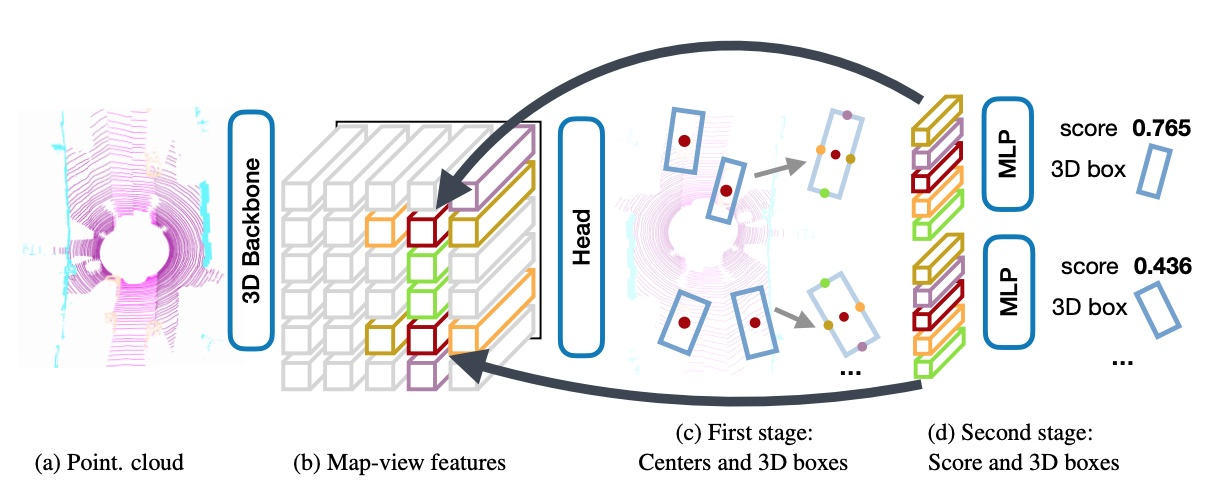
\includegraphics[width=0.75\linewidth]{Figures/centerpoint.jpg}
		\caption{CenterPoint network architecture}
		\label{fig:centerpoint}
	\end{figure}
	
	\subsubsection{BEVDet}
	BEVDet is a 3D object detection model that takes multi-camera images as input. The model first extracts image-view features, densely predicts pixel-wise depth, and converts the images into point clouds. Then, a pooling operation along the vertical (Z) axis aggregates these depth-aware features into a BEV feature map. Finally, a BEV encoder and detection head, partially based on the CenterPoint model, predict 3D object locations and attributes.
	\begin{figure}[H]
		\centering
		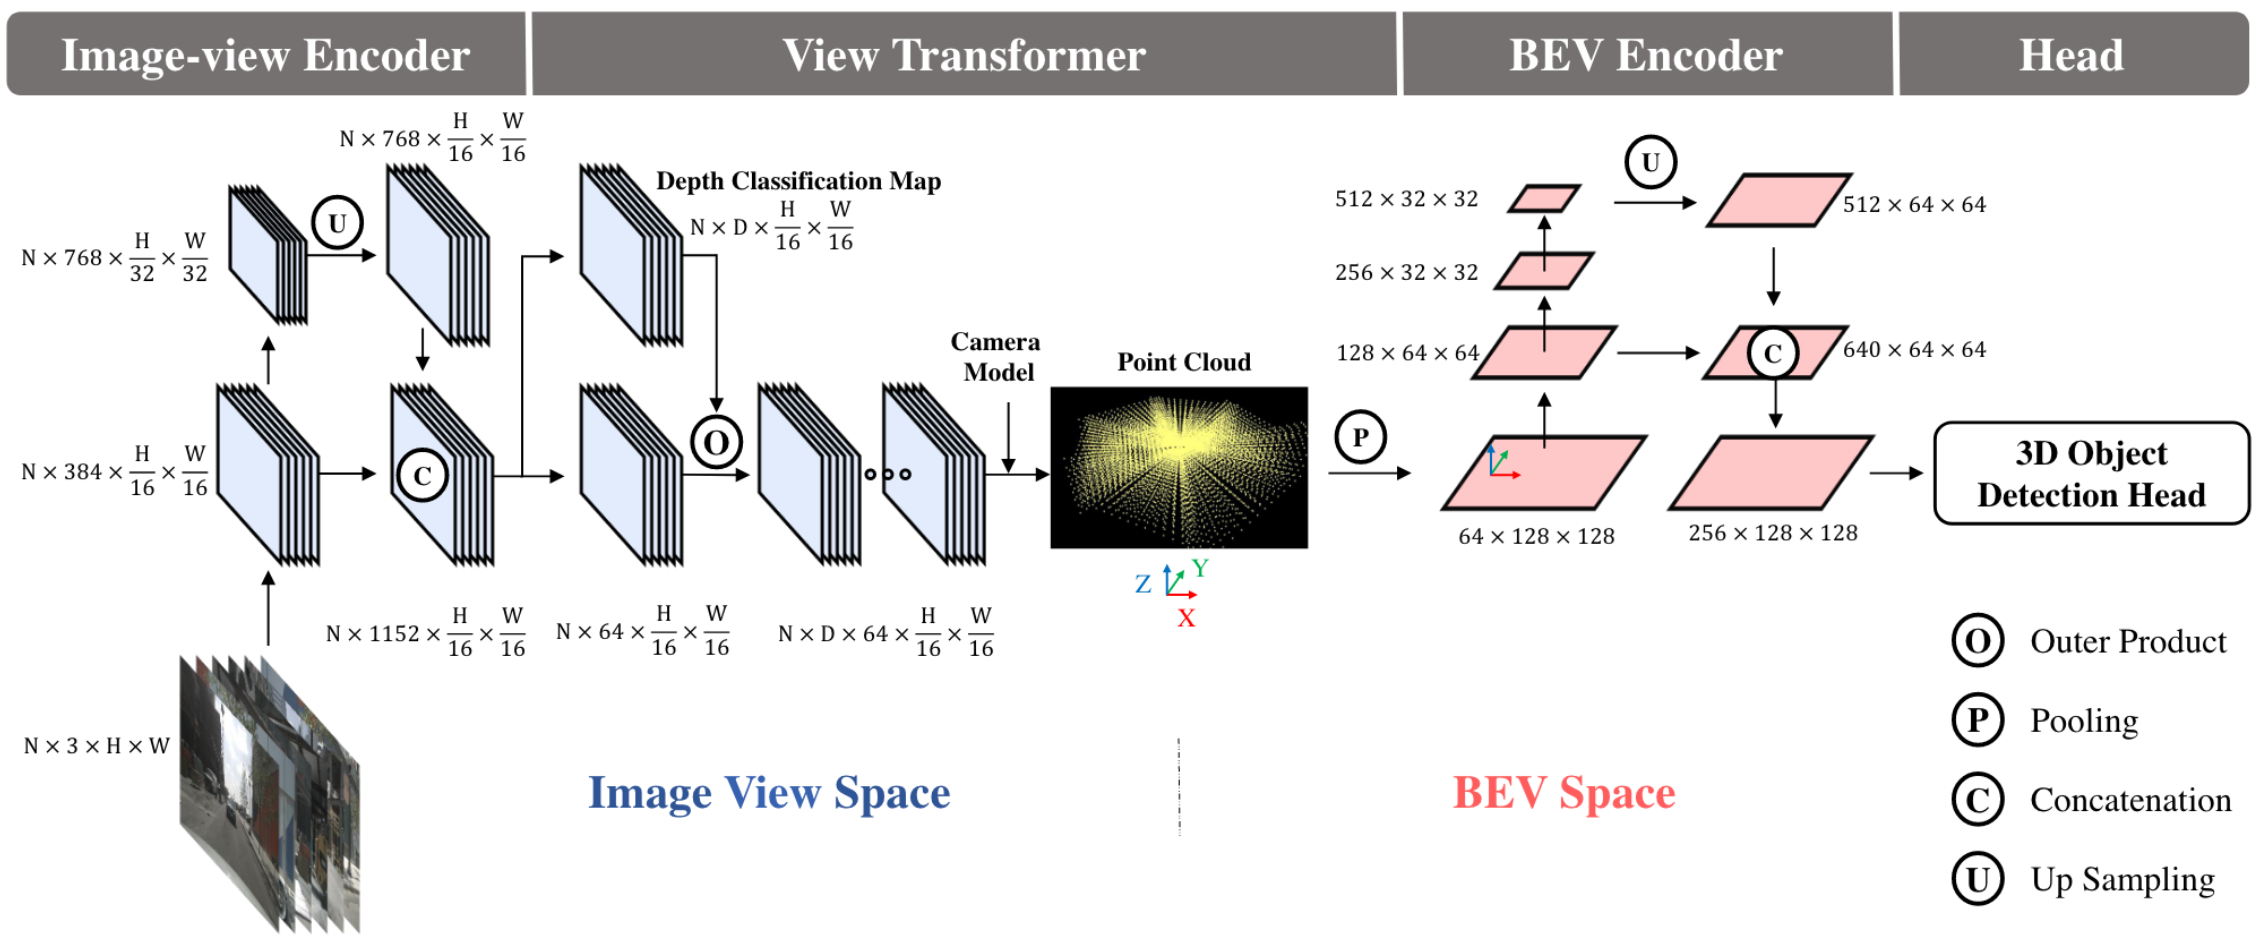
\includegraphics[width=0.75\linewidth]{Figures/bevdet.png}
		\caption{BEVDet network architecture}
		\label{fig:bevdet}
	\end{figure}
	
	Since BEVDet indirectly predicts the pixel depths, its effectiveness largely depends on the accuracy of depth estimation and the quality of BEV feature generation. Errors in depth prediction can propagate through the pipeline, affecting the final 3D object detection performance. However, by leveraging multi-camera inputs, BEVDet can potentially capture richer semantic information compared to LiDAR, which primarily provides geometric data. This additional visual context may enhance object recognition and provide better visual features where fine-grained appearance details are important.
	
	
	%We include a very simple multimodal baseline that ... ignores history... doesn't have attention ... doesn't require pretraining ....
	%(these are implemented by the group)
	
	\subsection{\points{0.5} Competitive Baselines}
	We run $2$ competitive baselines available at public repos.  These include: 
	(these are models you found in the literature, github, etc with existing checheckpoints -- no training. You should be able to run these so you can do analysis on them in R3.  Additionally, they need to be rerun if you've done your own data sampling)
	
	\begin{enumerate}
		\item Competitive Baseline 1 is MSMDFusion \cite{Jiao2022MSMDFusionFL}+BUTD \cite{Anderson2017BottomUpAT} whose key insight is using BUTD as QA head which advocates for computing bottom-up and top-down attention on salient regions of the image. Bottom-up attention detects salient image regions using a Faster R-CNN object detector, while top-down attention learns to reason over these regions based on the input question, enabling fine-grained grounding between visual content and language.
		
		\begin{figure}[H]
			\centering
			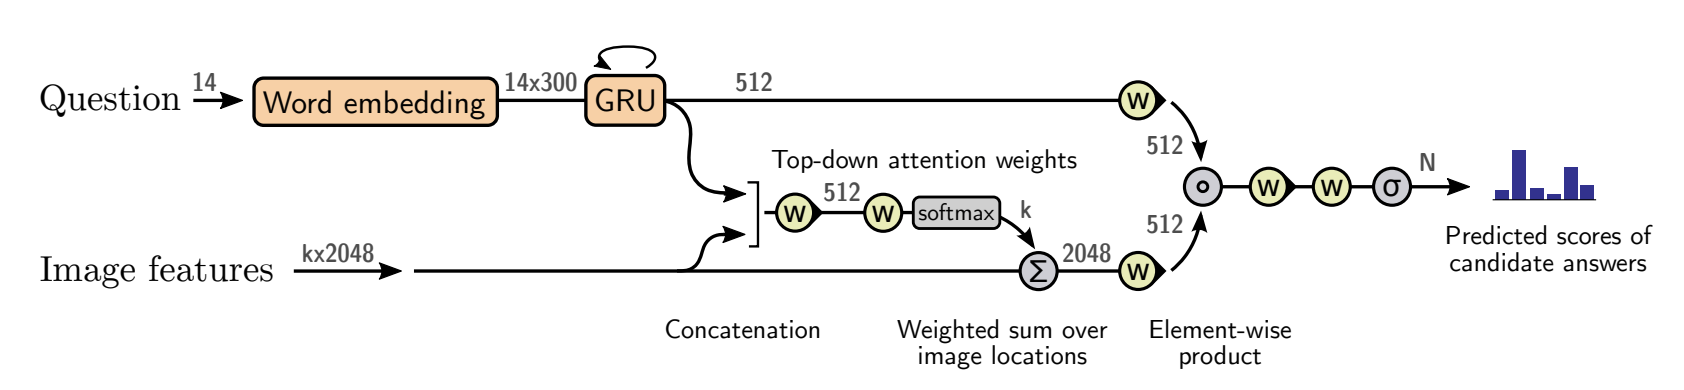
\includegraphics[width=0.75\linewidth]{Figures/BUTD Framework.png}
			\caption{BUTD network architecture}
			\label{fig:butd}
		\end{figure}
		
		
		\item Competitive Baseline 2 is MSMDFusion+MCAN \cite{Yu2019DeepMC} whose key insight is using MCAN as head which stacks self-attention and cross-attention modules for vision-language feature interaction. MCAN employs Modular Co-Attention to dynamically fuse image features and question embeddings at multiple levels, allowing the model to iteratively refine its understanding of both modalities. This hierarchical reasoning mechanism helps capture fine-grained alignments between visual objects and linguistic cues. 
	\end{enumerate}
	
	\begin{figure}[H]
		\centering
		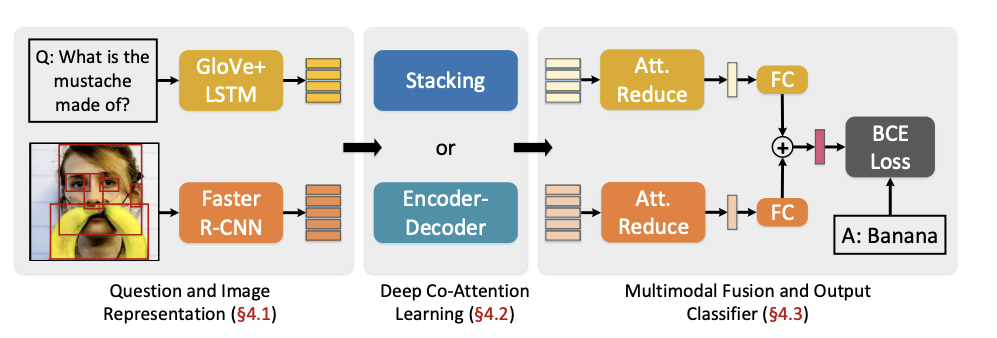
\includegraphics[width=0.75\linewidth]{Figures/MCAN Framework.png}
		\caption{MCAN network architecture}
		\label{fig:mcan}
	\end{figure}
	
	\clearpage
	
	\begin{table}[ht]
		\centering
		\resizebox{\textwidth}{!}{%
			\begin{tabular}{lcccccccccccccccc}
				\toprule
				\textbf{Models} & \multicolumn{3}{c}{\textbf{Exist}} & \multicolumn{3}{c}{\textbf{Count}} & \multicolumn{3}{c}{\textbf{Object}} & \multicolumn{3}{c}{\textbf{Status}} & \multicolumn{3}{c}{\textbf{Comparison}} & \textbf{Acc} \\
				\cmidrule(lr){2-4} \cmidrule(lr){5-7} \cmidrule(lr){8-10} \cmidrule(lr){11-13} \cmidrule(lr){14-16}
				& H0 & H1 & All & H0 & H1 & All & H0 & H1 & All & H0 & H1 & All & H0 & H1 & All  \\
				\midrule
				Q-Only+BUTD               & 81.7 & 78.3 & 79.9 & 18.7 & 18.8 & 18.8 & 63.2 & 40.0 & 43.4 & 57.2 & 49.2 & 52.0 & 81.0 & 64.5 & 66.0 & 54.0 \\ 
				
				BEVDet+BUTD          & 87.2 & 80.6 & 83.7 & 21.7 & 20.0 & 20.9 & 69.4 & 45.2 & 48.8 & 55.0 & 50.5 & 52.0 & 76.1 & 66.8 & 67.6 & 57.0 \\
				CenterPoint+BUTD     & 87.3 & 80.8 & 83.8 & 21.6 & 20.2 & 20.9 & 67.7 & 43.5 & 47.0 & 67.7 & 51.1 & 54.7 & 76.6 & 65.1 & 66.1 & 56.8 \\
				MSMDFusion+BUTD      & 89.4 & 81.4 & 85.1 & 25.3 & 21.3 & 23.2 & 73.3 & 48.7 & 52.3 & 67.4 & 55.4 & 59.5 & 81.6 & 67.2 & 68.5 & 59.8 \\
				%GroundTruth+BUTD     & 98.9 & 87.2 & 92.6 & 76.8 & 38.7 & 57.5 & 99.7 & 71.9 & 76.0 & 98.8 & 81.9 & 87.6 & 98.1 & 76.1 & 78.1 & 79.2 \\
				\midrule
				Q-Only+MCAN               & 81.7 & 78.6 & 80.1 & 18.8 & 18.8 & 18.8 & 64.9 & 40.9 & 44.5 & 56.9 & 45.6 & 49.5 & 80.5 & 65.9 & 67.3 & 54.2 \\   
				
				BEVDet+MCAN          & 87.2 & 81.7 & 84.2 & 21.8 & 19.2 & 20.4 & 73.0 & 47.4 & 51.2 & 64.1 & 49.9 & 54.7 & 75.1 & 66.7 & 67.4 & 57.9 \\
				CenterPoint+MCAN     & 87.1 & 82.4 & 84.6 & 21.7 & 20.8 & 21.2 & 69.8 & 50.9 & 53.7 & 64.5 & 56.3 & 59.1 & 75.5 & 66.8 & 67.6 & 59.3 \\
				MSMDFusion+MCAN      & 89.0 & 82.3 & 85.4 & 23.4 & 21.1 & 22.2 & 75.3 & 50.6 & 54.3 & 69.0 & 56.2 & 60.6 & 78.8 & 68.8 & 69.7 & 60.4 \\
				%GroundTruth+MCAN     & 99.6 & 95.5 & 97.4 & 52.7 & 39.9 & 46.2 & 99.7 & 86.2 & 88.2 & 99.3 & 95.4 & 96.7 & 99.7 & 90.2 & 91.0 & 84.3 \\
				\bottomrule
			\end{tabular}
		}
		\caption{Top-1 accuracy across different question types in the NuScenes-QA test set. H0 denotes zero-hop and H1 denotes one-hop. ({\points{1} for formatted table. \points{1} Results for for N*2 approaches (N is number of teammates)})}
	\end{table}
	
	
	\begin{comment}
		\begin{table}[t]
			\centering
			\begin{tabular}{@{}lrr@{}}
				\toprule
				& \multicolumn{2}{c}{Dev} \\
				Methods                     & Accuracy $\uparrow$ & $L_2$ Error $\downarrow$  \\
				\midrule
				Unimodal 1 \cite{} & & \\
				Unimodal 2 \cite{} & & \\
				Unimodal 3 \cite{} & & \\
				\midrule
				Simple Multimodal 1 \cite{} & & \\
				Simple Multimodal 2 \cite{} & & \\
				Simple Multimodal 3 \cite{} & & \\
				\midrule
				Previous Approach 1 \cite{} & & \\
				Previous Approach 2 \cite{} & & \\
				Previous Approach 3 \cite{} & & \\
				\bottomrule
			\end{tabular}
			\label{sec:results}
			\caption{\points{1} for formatted table. \points{1} Results for for N*2 approaches (N is number of teammates)}
		\end{table}
	\end{comment}
	
	
	\section{Results (1 page)}
	%Replace columns with the correct metrics for your task (extrinsic). What are 
	%all the things you can measure, and why are they beneficial?
	\points{1} For three metrics
	
	\subsection{Metric 1: Overall Accuracy (Acc)}
	\textbf{Definition}: Measures the top-1 accuracy across all test samples, regardless of question type.
	
	\textbf{Why is it beneficial?}
	\begin{itemize}
		\item Provides a high-level evaluation of the model’s performance.
		\item Allows for direct comparison between different models.
		\item Ensures that models correctly answer a variety of question types.
	\end{itemize}
	
	\subsection{Metric 2: H0 and H1 Accuracy}
	\textbf{Definition}:
	\begin{itemize}
		\item \textbf{H0 (Zero-hop)}: Questions that can be answered directly from object detection (e.g., “\textit{Is there a car?}”).
		\item \textbf{H1 (One-hop)}: Questions that require reasoning over detected objects (e.g., “\textit{Is the pedestrian behind the truck?}”).
	\end{itemize}
	
	\textbf{Why is it beneficial?}
	\begin{itemize}
		\item Differentiates between direct perception (H0) and reasoning-based inference (H1).
		\item Highlights whether models struggle more with basic object recognition or higher-level reasoning.
		\item Helps in understanding how different architectures (e.g., CenterPoint, MSMDFusion) contribute to reasoning.
	\end{itemize}
	
	\subsection{Metric 3: Accuracy in 5 Question Categories}
	\textbf{Definition}: Measures accuracy across five specific question categories:
	\begin{enumerate}
		\item \textbf{Existence} – Does an object exist in the scene?
		\item \textbf{Counting} – How many objects are in the scene?
		\item \textbf{Object Classification} – What type of object is present?
		\item \textbf{Status Recognition} – What is the state of the object (e.g., moving or parked)?
		\item \textbf{Comparison} – How do objects compare (e.g., "\textit{Does the construction vehicle have the same status as the car?}")
	\end{enumerate}
	
	Each category has:
	\begin{itemize}
		\item \textbf{H0 Accuracy} (direct detection-based answers).
		\item \textbf{H1 Accuracy} (requires additional reasoning).
		\item \textbf{Overall Accuracy} (average across H0 and H1).
	\end{itemize}
	
	\textbf{Why is it beneficial?}
	\begin{itemize}
		\item Provides a fine-grained evaluation of model strengths and weaknesses.
		\item Helps identify whether a model is better at direct perception (H0) or relational reasoning (H1).
		\item Useful for diagnosing where multimodal fusion (e.g., LiDAR + Camera) improves performance.
	\end{itemize}
	
	\begin{comment}
		\paragraph{Metric 1}
		
		\paragraph{Metric 2}
		
		\paragraph{Metric 3}
	\end{comment}
	
	\clearpage
	\section{Model Proposal (1 page)}
	Include a diagram (e.g. labeled flow chart) of all modules.  This is not final!
	
	\subsection{\points{1.5} Overall model structure }
	
	\begin{figure}[H]
		\centering
		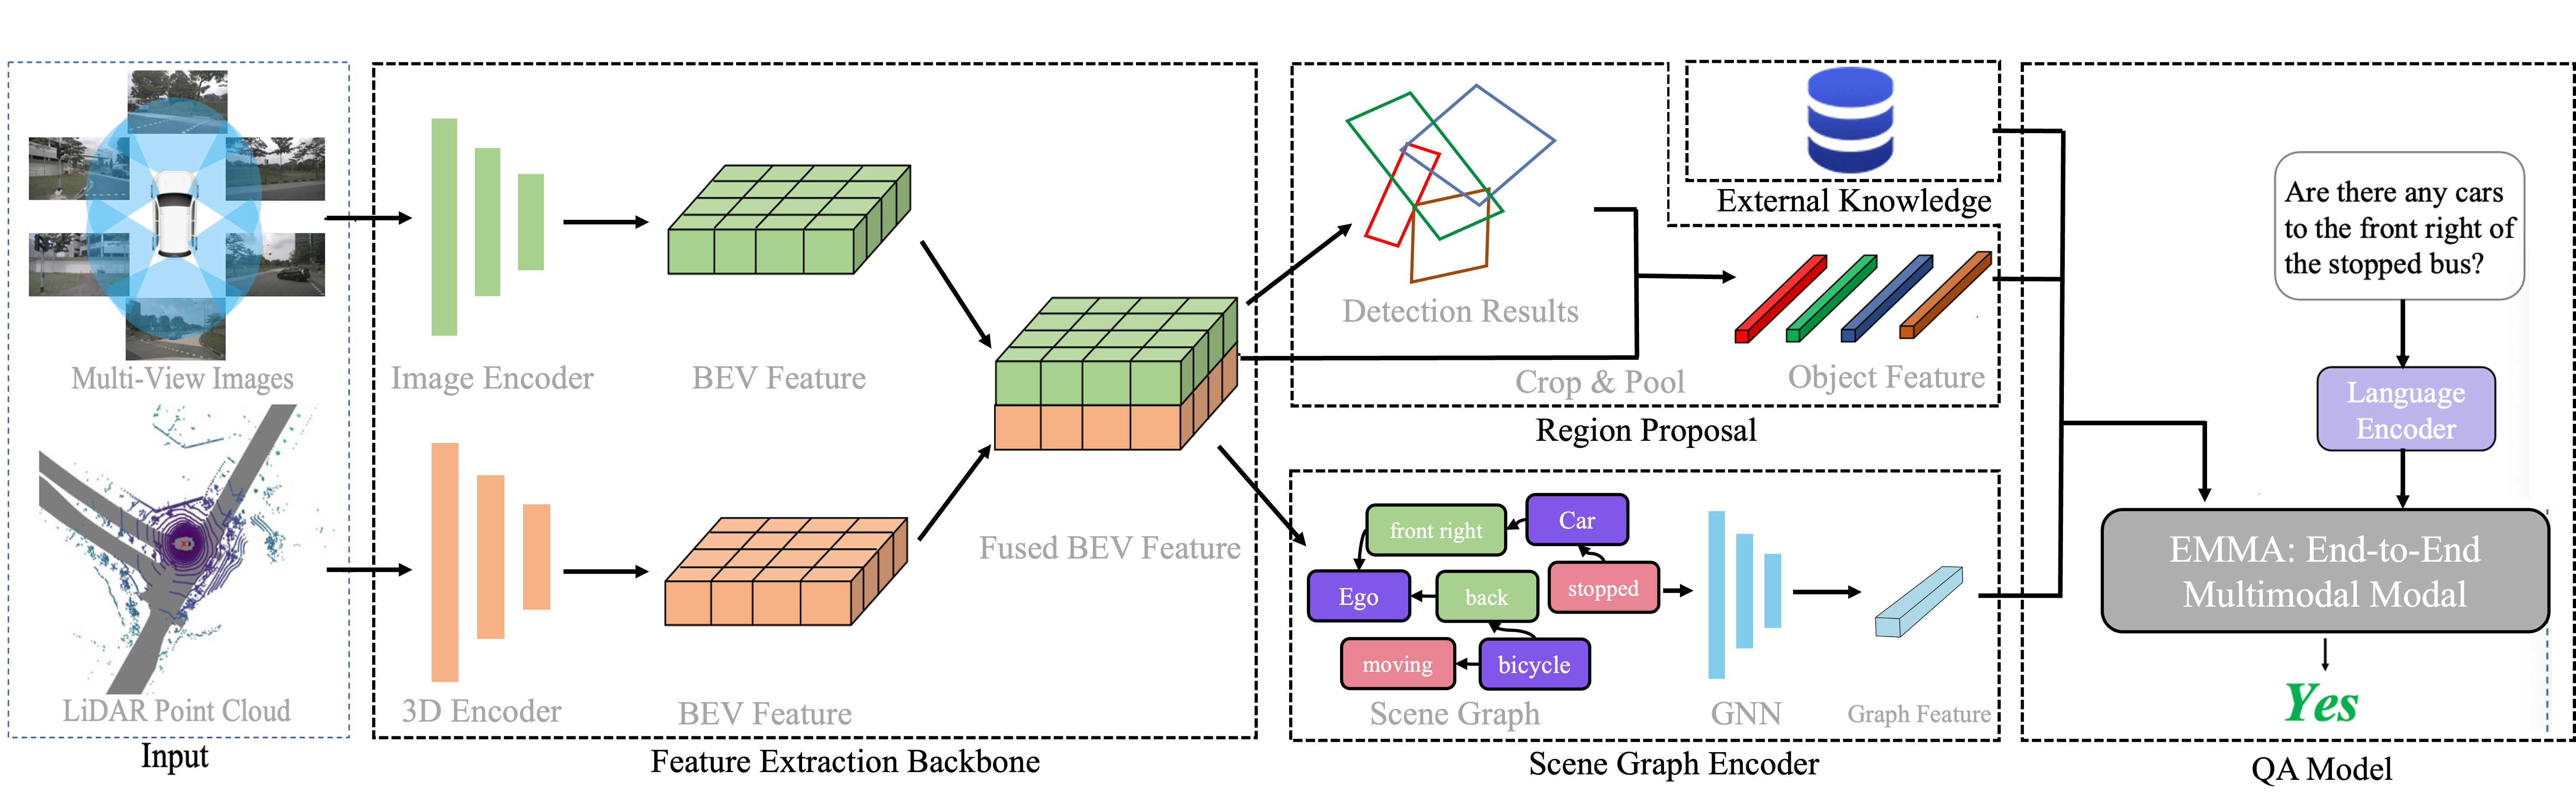
\includegraphics[width=\linewidth]{Figures/framework.png}
		\caption{Proposed Model Architecture}
		\label{fig:enter-label}
	\end{figure}
	
	The proposed model can be structured into four main components: the MSMDFusion encoder, scene graph encoder, external knowledge encoder, and QA model. Here's a detailed description of each component:
	
	\begin{enumerate}
		
		
		\item \textbf{MSMDFusion Encoder}: The MSMDFusion Encoder combines the functionalities of the Image Encoder and Point Cloud Encoder into a single, cohesive module. It processes both 2D visual data from multi-view cameras and 3D spatial data from LIDAR sensors, extracting and fusing features from these modalities into a unified Bird's Eye View (BEV) representation.
		
		\item \textbf{Scene Graph Encoder}: This branch focuses on understanding the relationships and interactions between different objects in the scene. It uses graph-based features and possibly a Graph Neural Network (GNN) to model the connections between objects. The scene graph encoder enhances the model's ability to interpret complex scenes by capturing contextual relationships.
		
		\item \textbf{External Knowledge Encoder}: The external knowledge encoder integrates additional contextual or domain-specific information to enrich the model's understanding. This could involve incorporating prior knowledge or external data sources to improve the accuracy and relevance of the model's predictions.
		
		\item \textbf{QA Model}: The QA (Question Answering) model is responsible for generating responses or predictions based on the integrated features from the image encoder, point cloud encoder, scene graph branch, and knowledge branch. It leverages the multimodal data to provide comprehensive answers or detection results, ensuring that the model can perform end-to-end tasks effectively.
	\end{enumerate}
	
	By organizing the model into these four components, it can effectively process and integrate multimodal data, leveraging both visual and spatial information to perform complex tasks such as object detection and scene understanding. The integration of graph-based features and external knowledge further enhances the model's capabilities, making it a robust end-to-end multimodal system.
	
	\subsection{\points{1} Encoders }
	%Describe encoders for each modality and at least one alternatives for each.  Explain the relative strengths of each option (e.g. coverage, efficiency, ...)
	
	\subsubsection{MSMDFusion Encoder}
	The MSMDFusion Encoder integrates multi-view camera images and LiDAR point clouds to enhance 3D object detection in autonomous driving. It consists of an image encoder (BEVDet-based) that extracts and projects 2D image features into Bird’s-Eye View (BEV) space, and a LiDAR encoder (CenterPoint-based) that processes 3D point clouds for precise object localization. By fusing multi-scale and multi-depth features, MSMDFusion improves detection accuracy, depth estimation, and spatial understanding in complex driving scenarios.
	
	\begin{figure}[H]
		\centering
		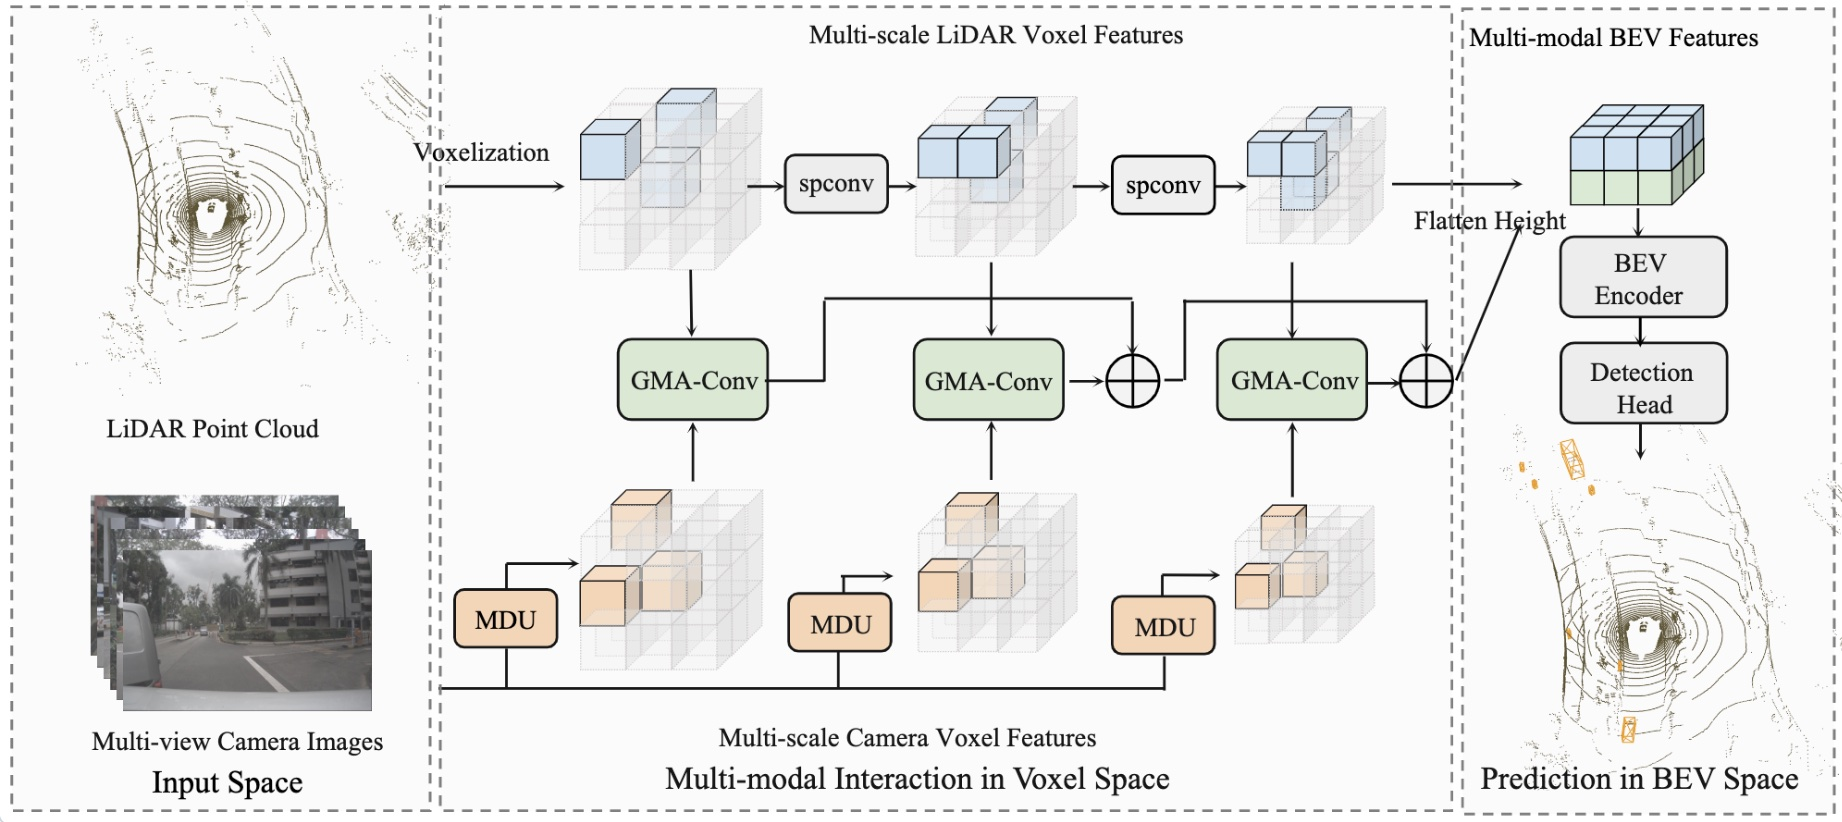
\includegraphics[width=0.75\linewidth]{Figures/msmdfusion.jpg}
		\caption{MSMDFusion Encoder}
		\label{fig:ekg}
	\end{figure}
	
	\subsubsection{Scene Graph Encoder}
	
	\begin{figure}[H]
		\centering
		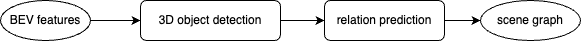
\includegraphics[width=0.8\linewidth]{Figures/scene-graph.png}
		\caption{Scene Graph Encoder}
		\label{fig:scene-graph}
	\end{figure}
	
	The Scene Graph Encoder, as shown in Fig. \ref{fig:scene-graph}, begins by utilizing an object detector to identify and localize all objects from the Bird's Eye View (BEV) features generated by the MSMDFusion Encoder. Once the objects are detected, the encoder predicts the relationships between every pair of objects, capturing contextual information such as spatial arrangements, interactions, and dependencies. 
	
	The ground truth for these relationships is derived from the annotations provided in the NuScenes-QA dataset, following the scene graph construction methods in \cite{qian2024nuscenes}. We define six relationships between objects, namely \textit{front}, \textit{back}, \textit{front left}, \textit{front right}, \textit{back left}, and \textit{back right}. To determine object relationships, we first project 3D bounding boxes onto the Bird’s-Eye-View (BEV). Subsequently, we calculate the angle between the vector connecting the centers of two bounding boxes and the forward direction of the ego-car. The formula is given by  
	
	\begin{equation}
		\theta = \cos^{-1} \left( \frac{(B_1[:2] - B_2[:2]) \cdot V_{ego}[:2]}{\| B_1[:2] - B_2[:2] \| \| V_{ego}[:2] \|} \right),
	\end{equation}
	
	where \( B_i = [x, y, z, x_{size}, y_{size}, z_{size}, \varphi] \) is the 3D bounding box of object \( i \), and \( V_{ego} = [v_x, v_y, v_z] \) represents the speed of the ego car. Based on the angle range, the relationship between two objects is defined as  
	
	\begin{equation}
		relation =
		\begin{cases}
			front, & \text{if } -30^\circ < \theta \leq 30^\circ \\
			front \ left, & \text{if } 30^\circ < \theta \leq 90^\circ \\
			front \ right, & \text{if } -90^\circ \leq \theta \leq -30^\circ \\
			back \ left, & \text{if } 90^\circ < \theta \leq 150^\circ \\
			back \ right, & \text{if } -150^\circ \leq \theta \leq -90^\circ \\
			back, & \text{else.}
		\end{cases}
	\end{equation}
	
	We define the forward direction of the car as \( 0^\circ \) and counterclockwise angles as positive. 
	
	
	\subsubsection{External Knowledge Encoder}
	
	The External Knowledge Encoder leverages a knowledge graph that captures general traffic rules and typical relationships between driving entities such as vehicles, cyclists, and pedestrians. Having explicitly structured rules helps in inferring right-of-way, identifying potential conflicts, and predicting plausible future behaviors based on traffic norms and spatial interactions. This graph can be generated from traffic rule databases, such as the MUTCD (Manual on Uniform Traffic Control Devices), the Highway Code (UK), and the Federal Motor Vehicle Safety Standards (FMVSS). The external knowledge extraction module retrieves relevant information from the graph, improving 3D object detection, trajectory forecasting, and question-answering tasks for autonomous systems.
	
	By incorporating the knowledge graph, we can enhance scene understanding by providing structured context to our multimodal large language model (MLLM), enabling the model to infer implicit traffic rules, predict interactions between entities, and reason about vehicles' status and intentions more reliably.
	\begin{figure}[H]
		\centering
		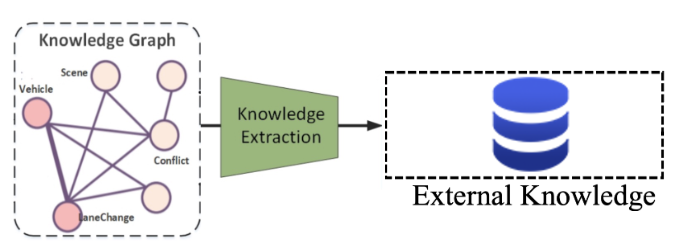
\includegraphics[width=0.55\linewidth]{Figures/knowledge_graph.png}
		\caption{External Knowledge Graph Encoder}
		\label{fig:ekg}
	\end{figure}
	
	
	
	
	\subsection{\points{1} Decoders }
	In our model, we use \textbf{OpenEMMA}\cite{Xing2024OpenEMMAOM} as our QA head that is decoder. OpenEMMA is the implementation of EMMA\cite{Hwang2024EMMAEM}. EMMA (End-to-End Multimodal Model for Autonomous Driving) is a novel end-to-end framework designed for autonomous driving, built on top of a multimodal large language model (MLLM). EMMA reframes driving tasks as visual question answering (VQA) problems, leveraging the extensive world knowledge and reasoning capabilities of pre-trained language models like Gemini. In EMMA, all non-sensor inputs (e.g., high-level navigation commands and vehicle status) and outputs (e.g., future trajectories, detected objects, and road graph elements) are represented as natural language text. This unified language space allows EMMA to jointly handle multiple driving-related tasks using task-specific prompts with Chain of Thoughts design.
	
	\begin{figure}[H]
		\centering
		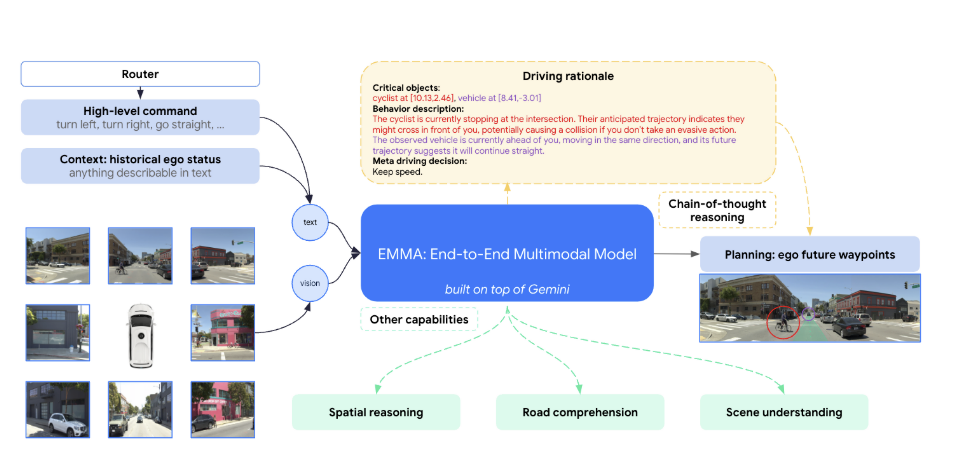
\includegraphics[width=0.9\linewidth]{Figures/EMMA Framework.png}
		\caption{OpenEMMA Model architecture}
		\label{fig:EMMA}
	\end{figure}
	
	OpenEMMA is an open-source end-to-end multimodal framework for autonomous driving, replicating the EMMA model. OpenEMMA leverages open soureced pre-trained Multimodal Large Language Models (MLLMs) combined with Chain-of-Thought reasoning to process front camera images and historical ego-vehicle status just EMMA did. To enhance object detection performance, OpenEMMA incorporates a fine-tuned YOLO3D model optimized for 3D bounding box estimation in driving scenarios. The system achieves state-of-the-art performance in trajectory planning and demonstrates strong generalizability across diverse and challenging driving scenes, showcasing EMMA’s potential ability in analyzing complex driving scenarios.
	
	
	
	
	\subsection{\points{1} Loss Functions }
	Describe both your primary task loss and three possible auxiliary losses that might improve performance.  Justify your choices.
	
	\textbf{OpenEMMA Loss Function}
	
	The OpenEMMA is trained on  multiple tasks with a single model as following:
	
	\begin{itemize}
		\item \textbf{Trajectory Prediction} 
		\\
		Trajectory prediction aims to forecast the future positions of the ego vehicle over a fixed time horizon. This task enables the vehicle to plan its motion while anticipating future maneuvers. The prediction is typically performed in the Bird’s Eye View (BEV) space, with each predicted waypoint representing the future (x, y) position at a given timestamp.
		
		Loss Function:
		The common loss function for trajectory prediction is the L2 loss between the predicted trajectory and the ground truth trajectory:
		
		$\mathcal{L}_{\text{traj}} = \frac{1}{T} \sum_{t=1}^{T} \left\| \mathbf{p}_t - \hat{\mathbf{p}}_t \right\|_2^2 $\text{where} \ \(\mathbf{p}_t\) and \(\hat{\mathbf{p}}_t\) are the ground truth and predicted coordinates at time \(t\), respectively, and \(T\) is the prediction horizon.
		
		
		\item \textbf{3D Object Detection} 
		\\
		3D object detection focuses on detecting traffic participants such as vehicles, pedestrians, and cyclists in the scene. The goal is to predict a 3D bounding box for each object, which includes position (x, y, z), dimensions (w, h, l), and orientation $\theta$. This task is critical for understanding the spatial layout of the scene.
		
		Loss Function:
		The loss for 3D object detection typically combines multiple components, including localization loss, size loss, and orientation loss:
		\[
		\mathcal{L}_{\text{3D}} = \mathcal{L}_{\text{cls}} + \lambda_1 \mathcal{L}_{\text{loc}} + \lambda_2 \mathcal{L}_{\text{size}} + \lambda_3 \mathcal{L}_{\text{yaw}}
		\]
		where:
		\begin{itemize}
			\item \(\mathcal{L}_{\text{cls}}\): Classification loss (e.g., focal loss) for object category.
			\item \(\mathcal{L}_{\text{loc}} = \left\| \mathbf{c} - \hat{\mathbf{c}} \right\|_1\) for 3D center coordinates.
			\item \(\mathcal{L}_{\text{size}} = \left\| \mathbf{s} - \hat{\mathbf{s}} \right\|_1\) for object size.
			\item \(\mathcal{L}_{\text{yaw}}\): Orientation loss (e.g., smooth L1 or sine-cosine regression).
		\end{itemize}
		\item \textbf{Road Graph Estimation} 
		\\
		Road graph estimation is a structured prediction task that reconstructs the road topology in the scene. This involves predicting a set of unordered polylines, each represented as a sequence of waypoints, which collectively form the drivable lanes and road boundaries. Evaluation uses two levels:
		\begin{itemize}
			\item Lane-level precision and recall: True positives are polylines that match a ground truth polyline within a Chamfer distance threshold (1 meter).
			\item Pixel-level precision and recall: Both predicted and ground truth polylines are rasterized into a BEV grid (1m resolution), and matching is done per-pixel.
		\end{itemize}
		Loss Function:
		The loss can be formulated as a combination of Chamfer Distance Loss (for polyline matching) and Binary Cross Entropy (BCE) (for rasterized segmentation map):
		
		\[
		\mathcal{L}_{\text{road}} = \mathcal{L}_{\text{chamfer}} + \lambda \mathcal{L}_{\text{bce}}
		\]
		
		\begin{itemize}
			\item Chamfer Distance Loss between predicted and ground truth polylines:
			\[
			\mathcal{L}_{\text{chamfer}} = \frac{1}{N} \sum_{p \in \hat{\mathcal{P}}} \min_{q \in \mathcal{P}} \|p - q\|_2 + \frac{1}{M} \sum_{q \in \mathcal{P}} \min_{p \in \hat{\mathcal{P}}} \|p - q\|_2
			\]
			where \(\hat{\mathcal{P}}\) and \(\mathcal{P}\) denote predicted and ground truth polylines.
			
			\item BCE loss for rasterized BEV grid:
			\[
			\mathcal{L}_{\text{bce}} = - \frac{1}{HW} \sum_{i=1}^{H}\sum_{j=1}^{W} \left( y_{ij}\log(\hat{y}_{ij}) + (1 - y_{ij})\log(1 - \hat{y}_{ij}) \right)
			\]
		\end{itemize}
		
		
		
		
		\item \textbf{Scene Understanding (Temporary Blockage Detection)}
		\\
		Scene understanding focuses on understanding the semantic meaning of the current driving scene. A key sub-task is temporary blockage detection, where the model determines whether a lane is temporarily blocked. This is framed as a binary classification task (“blocked” or “not blocked”). The model is typically pre-trained on related tasks (like road graph estimation) to enhance its contextual understanding before fine-tuning on this specific classification task.
		
		Loss Function:
		The loss for this binary classification task is simply:
		\[
		\mathcal{L}_{\text{scene}} = - \frac{1}{N} \sum_{i=1}^{N} \left( y_i \log \hat{y}_i + (1 - y_i)\log (1 - \hat{y}_i) \right)
		\]
		
		where \(y_i\) is the ground truth label (1 for blocked, 0 for not blocked), and \(\hat{y}_i\) is the predicted probability.
	\end{itemize}
	
	\bibliography{references}
	\bibliographystyle{iclr2024_conference}
	
	\appendix
	\section{Appendix}
	You may include other additional sections here.
	
\end{document}